\documentclass[handout]{beamer}
\usepackage[english]{babel}
\usepackage{csquotes}
\usepackage[backend=biber,style=apa,sorting=none]{biblatex}
\addbibresource{references.bib}
\usetheme{Madrid}

\author{Thijs Raymakers}
\title{Progress presentation}
\date{May 13, 2020}

\begin{document}

\begin{frame}
    \titlepage
\end{frame}

\section{Context}
\begin{frame}
\frametitle{Context}
\begin{itemize}
    \item Gender bias is present in word embeddings~\footfullcite{bolukbasi_2016_quantifying_stereotypes}
    \pause
    \item Interesting to look at different languages
    \pause
    \item Showing which languages have a gender bias
    \pause
    \begin{block}{Research question}
        Do word embeddings of different languages have a different gender bias?
    \end{block}
    \pause
    \item Enables future research to look into exact differences
\end{itemize}
\end{frame}

\section{Current experiment}
\begin{frame}
    \frametitle{Current experiment}
    \begin{itemize}
        \item To calculate the ``bias" of a word \textit{x}
        \begin{itemize}
            \item Calculate the cosine distance between \textit{x} and \textit{man}
            \item Calculate the cosine distance between \textit{x} and \textit{woman}
            \item Calculate the difference between the two 
        \end{itemize}
        \pause
        \item If difference is close to zero, the word is equally associated with both \textit{man} and \textit{woman}
        \item Otherwise, it is more associated with either \textit{man} or \textit{woman}
        \pause
        \item This is done for all words in word embeddings of 26 languages from 16 different language families.
    \end{itemize}
\end{frame}

\section{Preliminary Results}
\begin{frame}
    \frametitle{Preliminary Results}
    \begin{columns}[T]
        \begin{column}{6cm}
            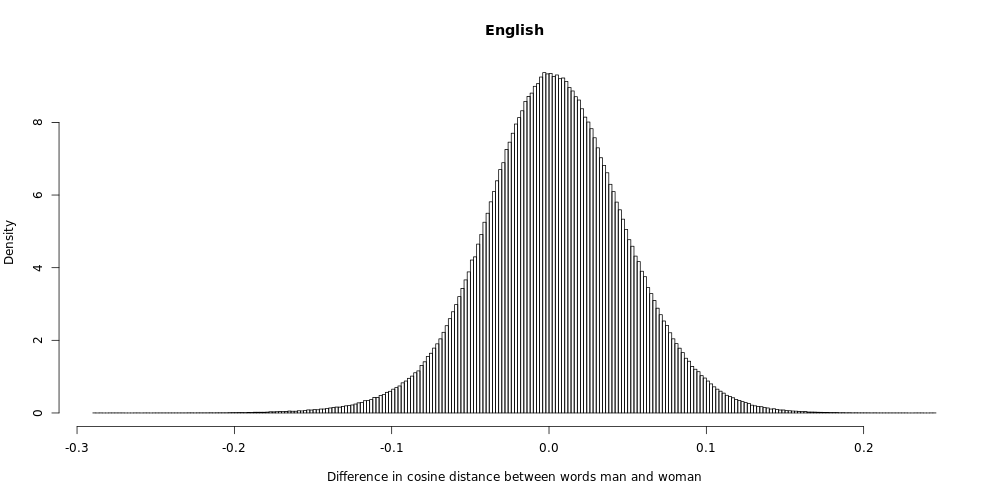
\includegraphics[width=7cm]{images/en_hist.png}
            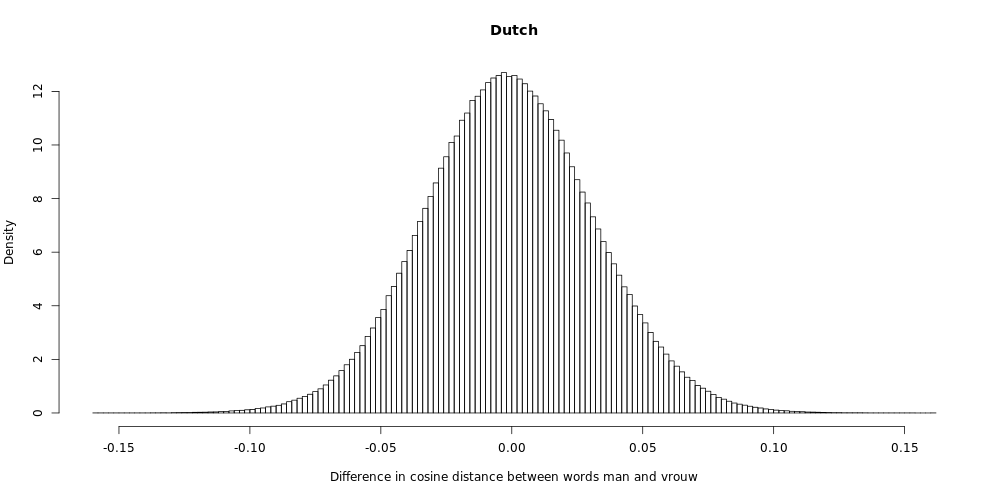
\includegraphics[width=7cm]{images/nl_hist.png}
        \end{column}
        \begin{column}{6cm}
            \begin{itemize}
                \item Both Indo-European, Germanic languages
                \pause
                \item Mean is close to 0
                \pause
                \item Variance of of English is larger
            \end{itemize}
        \end{column}
    \end{columns}
\end{frame}

\begin{frame}
    \frametitle{Preliminary Results}
    \begin{columns}[T]
        \begin{column}{6cm}
            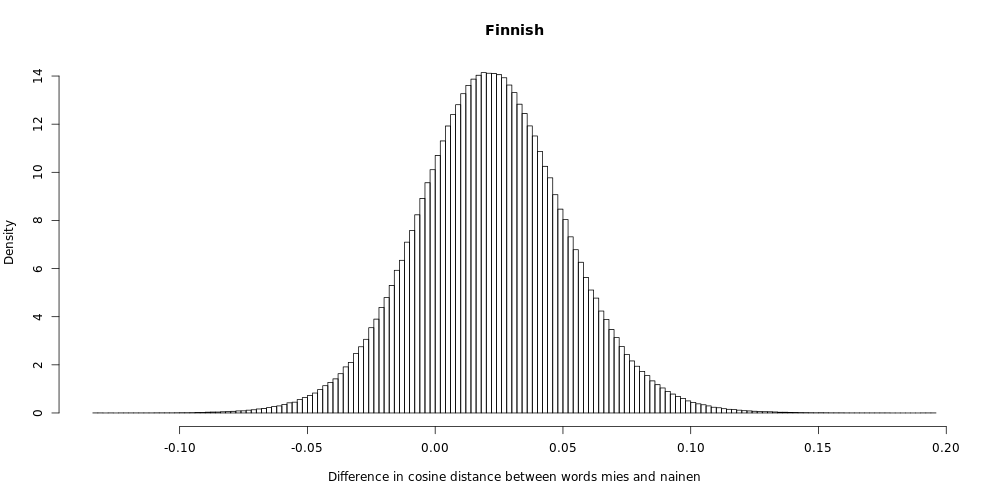
\includegraphics[width=7cm]{images/fi_hist.png}
            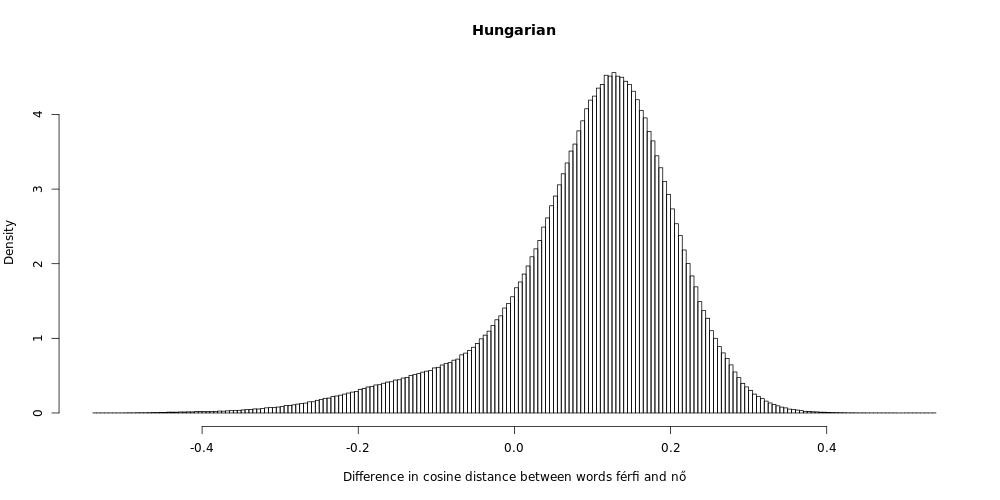
\includegraphics[width=7cm]{images/hu_hist.png}
        \end{column}
        \begin{column}{6cm}
            \begin{itemize}
                \item Both part of Uralic language family
                \item Mean is above zero, might indicate bias against women
            \end{itemize}
        \end{column}
    \end{columns}
\end{frame}

\begin{frame}
    \frametitle{Preliminary Results}
    \begin{columns}[T]
        \begin{column}{6cm}
            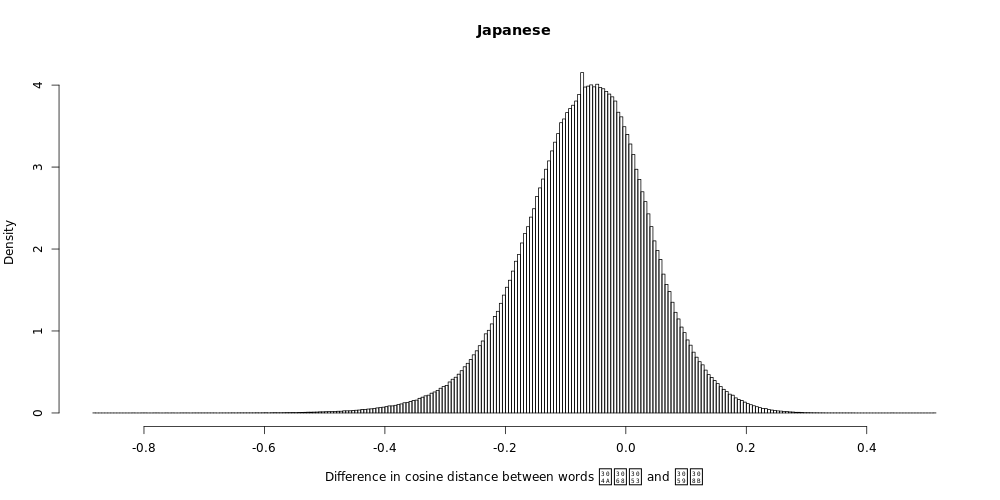
\includegraphics[width=7cm]{images/ja_hist.png}
            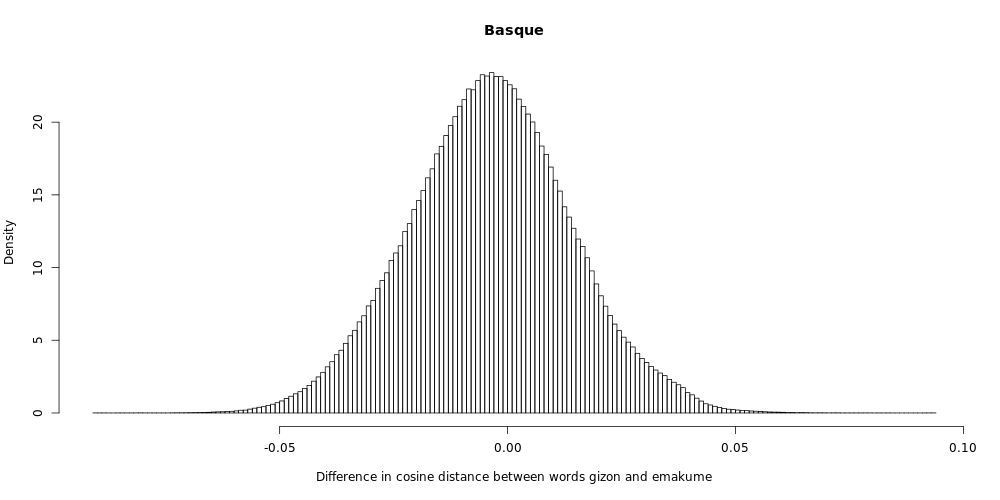
\includegraphics[width=7cm]{images/eu_hist.png}
        \end{column}
        \begin{column}{6cm}
            \begin{itemize}
                \item Both fairly isolated languages
                \item Mean is below zero, might indicate bias against men
            \end{itemize}
        \end{column}
    \end{columns}
\end{frame}

\section{Current issues / planning}
\begin{frame}
    \frametitle{Current issues / planning}
    \begin{itemize}
        \item Finding and understanding a way to statistically measure if difference 
            is significant
            \begin{itemize}
                \item Languages do not have the same distribution
                \item Almost 45M datapoints in total, 1.7M per language
                \item Currently looking at ANOVA, Kolmogorov-Smirnov test, Mann-Whitney U test and permutation test 
            \end{itemize}
    \end{itemize}
\end{frame}

%\section{References}
%\begin{frame}
%\frametitle{References}
%\printbibliography[heading=none]
%\end{frame}

\end{document}

